\subsection{Testing for SQL Injection - OTG-INPVAL-005}\label{sql_injection}
\subsubsection{BANK-APP}
\begin{tabular*}{\textwidth}{ p{.20\textwidth} | p{.75\textwidth} }\hline
    & \textbf{BANK-APP} \\ \hline
    \textbf{Observation} & The field \code{recipient} in the transaction form is vulnerable to SQL injection. \\
    \textbf{Discovery} & The login, registration and make transaction sites were tested for SQL injection with \code{sqlmap}. The command used for testing the login is \code{sqlmap -u "http://IP\_ADDRESS/secure-coding/public/\allowbreak login.\allowbreak php" -{}-data=\allowbreak "email=test\&password=test"}. For testing the transaction the session cookie has to be given as an extra parameter in the command as \code{-{}-cookie="PHPSESSID=cookie"}. \\
    \textbf{Likelihood} & what is the likelihood that this vulnerability is exploited? Which assumptions must hold and which skills must an attacker have? \\
    \textbf{Impact} & what is the potential impact of an exploit of this vulnerability? What could happen? \\
    \textbf{CVSS} &
        \begin{tabular}{l | l}
            Attack Vector           & \textcolor{red}{Network} \\
            Attack Complexity       & \textcolor{Green}{High} \\
            Privileges Required     & \textcolor{BurntOrange}{Low} \\
            User Interaction        & \textcolor{red}{None} \\
            Scope                   & \textcolor{red}{Unchanged} \\
            Confidentiality Impact  & \textcolor{red}{High} \\
            Integrity Impact        & \textcolor{red}{High} \\
            Availability Impact     & \textcolor{red}{High}
        \end{tabular}
    \\ \hline
\end{tabular*}

\subsubsection{SecureBank}
\begin{tabular*}{\textwidth}{ p{.20\textwidth} | p{.75\textwidth} }\hline
    & \textbf{SecureBank} \\ \hline
    \textbf{Observation} & Testing for SQL injection all pages were safe. \\
    \textbf{Discovery} & The login, registration and make transaction sites were tested for SQL injection with \code{sqlmap}. The command used for testing the login is \code{sqlmap -u "http://\allowbreak IP\_ADDRESS/login" -{}-data=\allowbreak "form\_login\allowbreak [email]=test\&form\_login\allowbreak [password]=test"}. For testing the transaction the session cookie has to be given as an extra parameter in the command as \code{-{}-cookie="Main\_session=cookie"}. \\
    \textbf{Likelihood} & N/A \\
    \textbf{Impact} & N/A \\
    \textbf{CVSS} & N/A \\ \hline
\end{tabular*}

\subsubsection{Comparison}
BANK-APP is vulnerable to SQL injection on the transaction page in the field \code{recipient}. Figure~\ref{fig:sql_vuln} shows the result of \code{sqlmap} for BANK-APP. If a page is not vulnerable for SQL injection, the result looks like the one in figure~\ref{fig:sql_safe}. All the pages for SecureBank were not vulnerable.

\begin{figure}[ht]
	\centering
	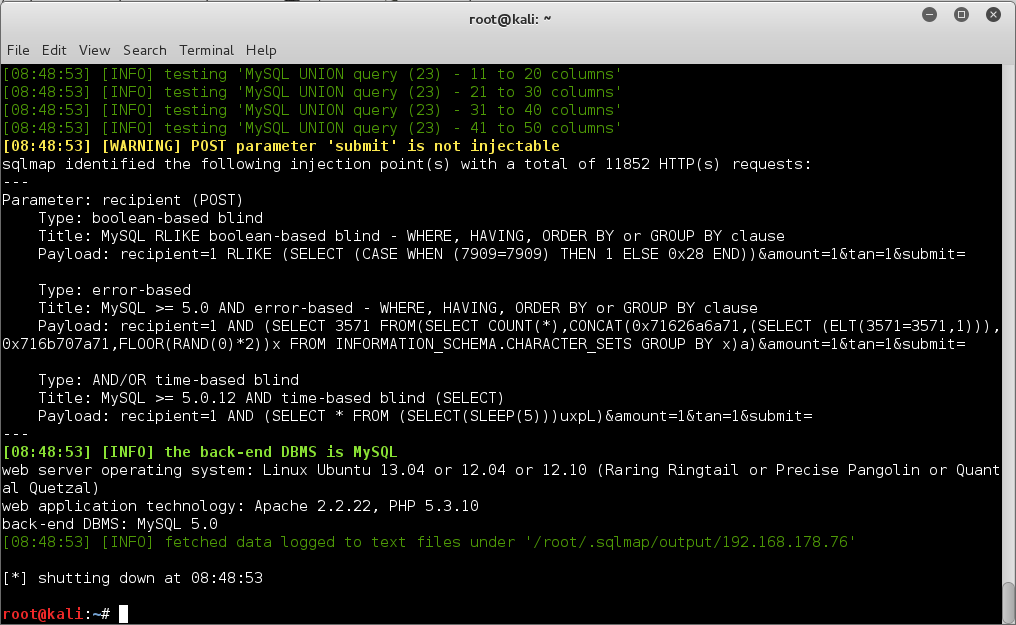
\includegraphics[width=.8\linewidth]{figures/OTG-INPVAL-005_1.png}
	\caption{\code{sqlmap} command shows vulnerability for SQL injection for BANK-APP}
	\label{fig:sql_vuln}
\end{figure}

\begin{figure}[ht]
	\centering
	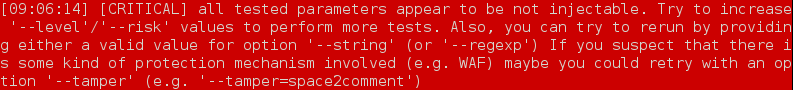
\includegraphics[width=.8\linewidth]{figures/OTG-INPVAL-005_2.png}
	\caption{\code{sqlmap} result if page is not vulnerable for SQL injection}
	\label{fig:sql_safe}
\end{figure}

\clearpage